\section{Data}
\label{sec:data}

\subsection{DESI imaging LRG sample}
Our sample of LRGs is drawn from the DESI Legacy Imaging Surveys Data Release 9 \citep[DR9;][]{dey2018overview} using the color-magnitude selection criteria designed for the DESI 1\% survey \mr{(CITE)}, described as the SV3 selection in more detail in \cite{zhou2022target}. The color-magnitude selection cuts are defined in the $g$, $r$, $z$ bands in the optical and $W1$ band in the infrared, as summarized in Tab. \ref{tab:ts}. The selection cuts are developed differently for each imaging survey to reach an almost uniform target surface density despite different survey efficiency and photometric calibration between DECaLS and BASS+MzLS. The implementation of these selection cuts in the DESI data processing pipeline is explained in \cite{myers2022}. Fig. \ref{fig:nz} shows the redshift distribution of the DR9 LRGs (solid black), inferred from the spectroscopic DESI Survey Validation data \mr{(CITE)}, and the evolution of halo bias (red dashed), adopted from \cite{zhou2021clustering}.

\begin{figure}
 \centering
 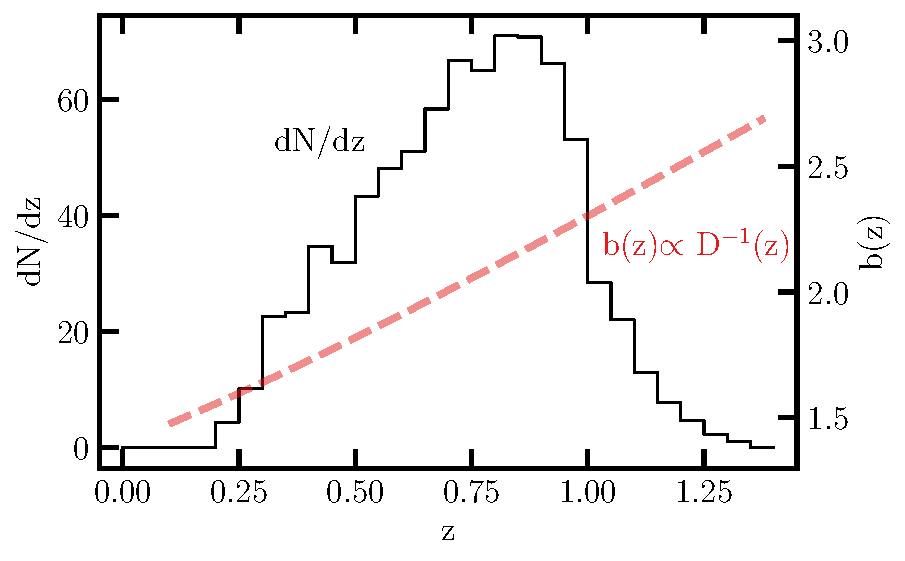
\includegraphics[width=0.5\textwidth]{figures/nz_lrg.pdf}
 \caption{The redshift distribution (solid) and bias evolution (dashed) of the DR9 LRG sample. The redshift distribution is determined by DESI spectroscopy, and the model for bias assumes a constant clustering amplitude \citep[see, e.g.,][]{zhou2021clustering, zhou2022target}.}
 \label{fig:nz}
\end{figure}

\begin{table*}
\caption{Selection criteria for the DESI-like LRG targets \citep{zhou2022target}. Magnitudes are corrected for MW extinction. $z_{\rm fiber}$ represents the z-band fiber magnitude which corresponds to the expected flux within a DESI fiber.} \label{tab:ts}
 \centerline{%
 \begin{tabular}{lll}
 \hline
 \hline
 \textbf{Footprint} & \textbf{Criterion} &\textbf{Description}\\
 \hline
 \hline  
 & $z_{\rm fiber} < 21.7$ & Faint limit \\
  DECaLS & $z - W1 > 0.8 \times (r - z) - 0.6$ & Stellar rejection \\
 & $[(g-r >1.3)~{\rm AND}~((g-r) > -1.55*(r-W1) + 3.13)]~{\rm OR}~(r -W 1 > 1.8)$ & Remove low-z galaxies \\
 & $[(r-W1 > (W1 - 17.26)*1.8)~{\rm AND}~(r - W1 > W1 - 16.36)]~{\rm OR}~(r-W1 > 3.29)$ & Luminosity cut \\ 
 \hline
 & $z_{\rm fiber} < 21.71$ & Faint limit \\
 BASS+MzLS & $z - W1 > 0.8 \times (r - z) - 0.6$ & Stellar rejection \\
 & $[(g-r >1.34)~{\rm AND}~((g-r) > -1.55*(r-W1) + 3.23)]~{\rm OR}~(r -W 1 > 1.8)$ & Remove low-z galaxies \\
 & $[(r-W1 > (W1 - 17.24)*1.83)~{\rm AND}~(r - W1 > W1 - 16.33)]~{\rm OR}~(r-W1 > 3.39)$ & Luminosity cut \\ 
 \hline
 \end{tabular}}
\end{table*}

\begin{figure*}
 \centering
 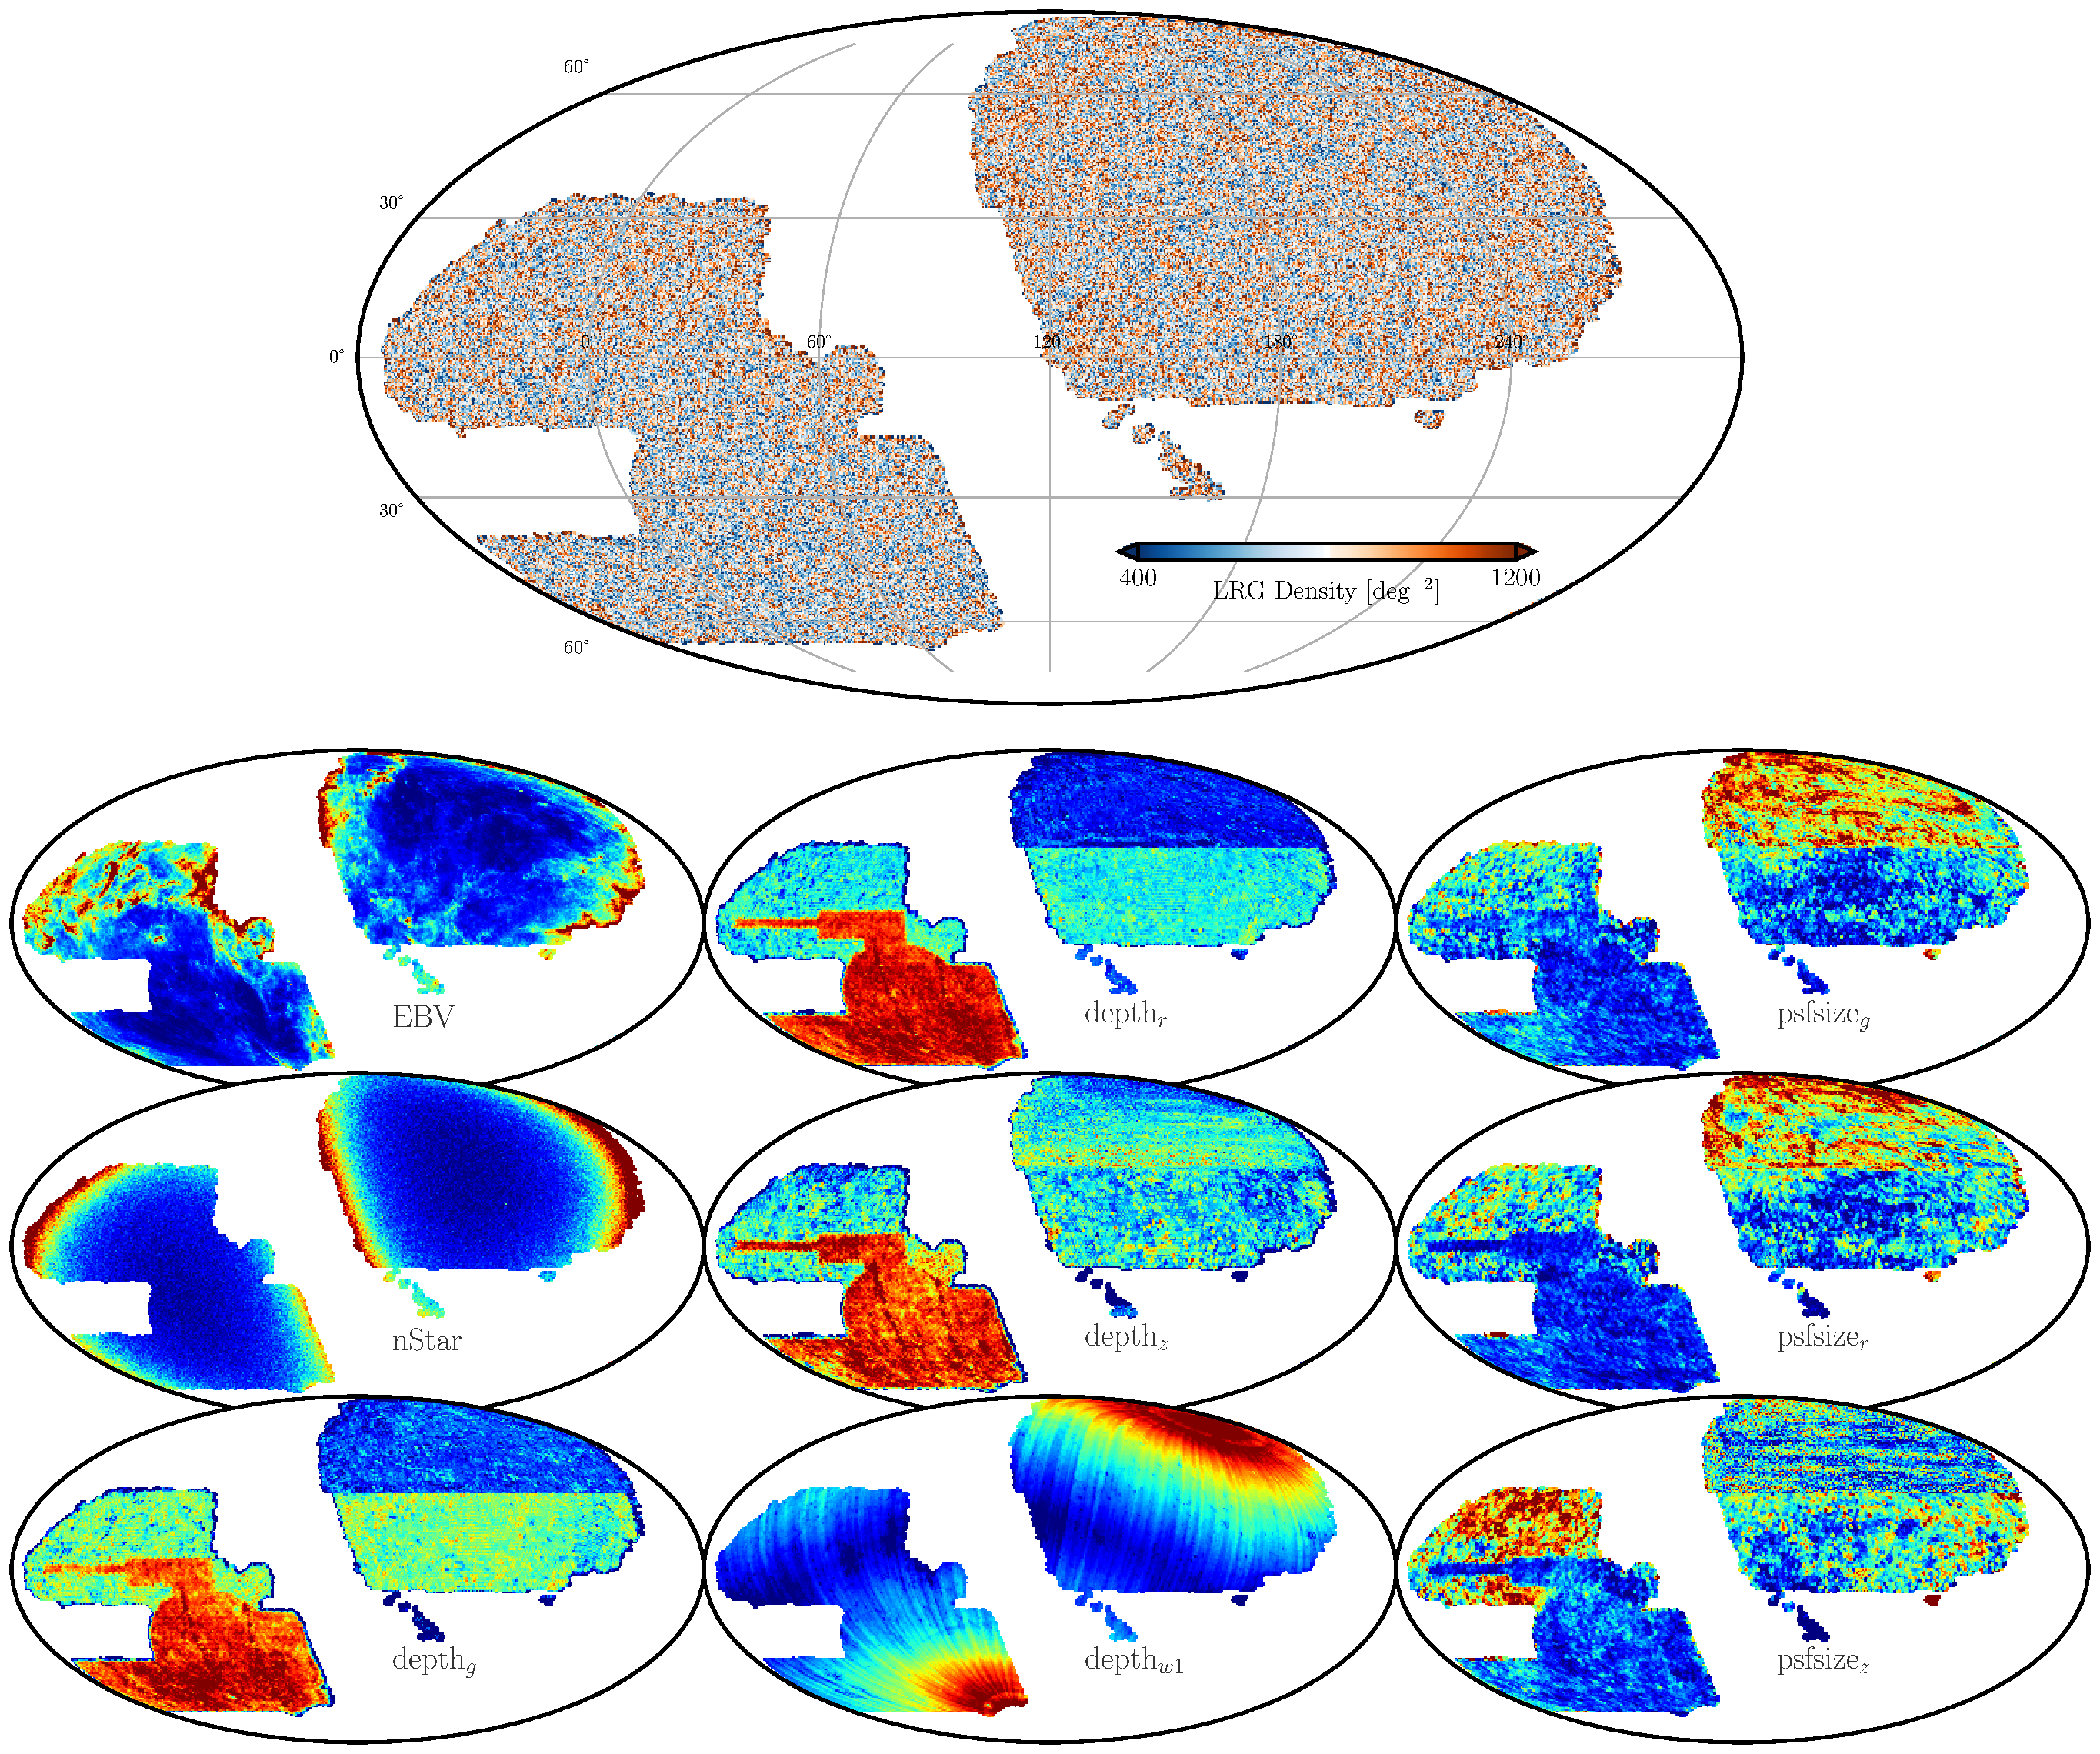
\includegraphics[width=0.95\textwidth]{figures/dr9data.pdf}
 \caption{Top: The DESI imaging LRG density field in Mollweide projection. Spurious disconnected islands from the North footprint and declination below $-30$ from the South footprint are removed for the analysis due to potential calibration issues (see text). Bottom: Mollweide projections of the DR9 catalog imaging properties (survey depth and astronomical seeing/psfsize) and MW foregrounds (extinction and local stellar density) in celestial coordinates.}
 \label{fig:ng}
\end{figure*}

DESI-like LRGs are selected brighter than the imaging survey depth limits; therefore, the DR9 LRG density field is nearly homogenous, unlike the other DESI tracers. To further reduce stellar contamination, the LRG sample is masked rigorously for foreground bright stars, galaxies, and clusters of galaxies\footnote{See the maskbits at \url{https://www.legacysurvey.org/dr9/bitmasks/}}. Then, the sample is binned into \textsc{HEALPix} \citep{gorski2005healpix} pixels at $\textsc{nside}=256$ to construct the 2D density map with an average surface density of $800$ deg$^{-2}$ with sky coverage around $14000$ square degrees. We correct for the pixel incompleteness and lost areas in the LRG density field using a catalog of random points, hereafter referred to as randoms, uniformly scattered over the footprint with the same cuts and masks applied. Fig. \ref{fig:ng} (top) shows the observed density field of the DR9 LRGs in deg$^{-2}$ before applying any correction weights to account for imaging systematic effects. The DR9 LRG density exhibits large-scale spurious fluctuations, which are unlikely to be of cosmological origin. Specifically, the SGC footprint exhibits some systematic under-density while there is some systematic over-density near the survey boundaries in the NGC. 

\subsubsection{Correlation coefficients}
First, we study the linear correlation between the LRG density map and various imaging properties which are considered as potential sources of systematic error. The imaging properties are mapped into \textsc{HEALPix} pixels at the same \textsc{nside}. Following \cite{zhou2022target}, the imaging properties investigated in this work are local stellar density constructed from point-like sources with a g-band magnitude in the range $12 \leq g < 17$ from the Gaia DR2 \citep[see,][]{gaiadr2, myers2022}; Galactic extinction E[B-V] from \cite{schlegel1998maps}; and survey-related imaging properties include survey depth (galaxy depth in the $g$, $r$, and $z$ bands and PSF depth in W1) and astronomical seeing (psfsize) in the $g$, $r$, and $z$ bands. Templates for the survey-related imaging properties are produced by binning the randoms into \textsc{HEALPix},  and averaging over the imaging attributes of the randoms in each pixel. 

Fig. \ref{fig:ng} (bottom) illustrates the imaging templates investigated as potential sources of systematic error. Each map shows its own characteristic large-scale spurious fluctuations. For instance, the under-dense part of the DR9 LRG sample in the SGC can be associated with survey depth, while the over-density in the NGC can be linked to the extinction map. We reject some parts of the DR9 sample to minimize the potential for photometric calibration systematics. There are some disconnected islands, hereafter referred to as \textit{spurious islands}, in the DECaLS North region at Dec $< -11$. Additionally, some parts of the DECaLS South footprint with Dec $< -30$ are removed from the sample, because a different catalog of standard stars is employed to calibrate images below that region. We discuss how these quality cuts influence $\fnl$ constraints from the DR9 LRG sample in Section \ref{sec:results}. 

\begin{figure}
 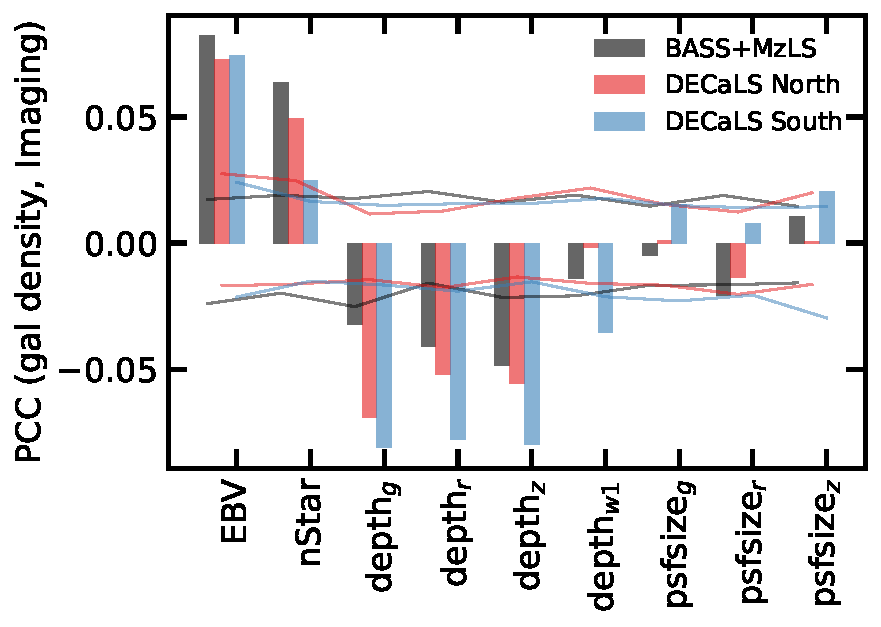
\includegraphics[width=0.5\textwidth]{figures/pcc.pdf} 
 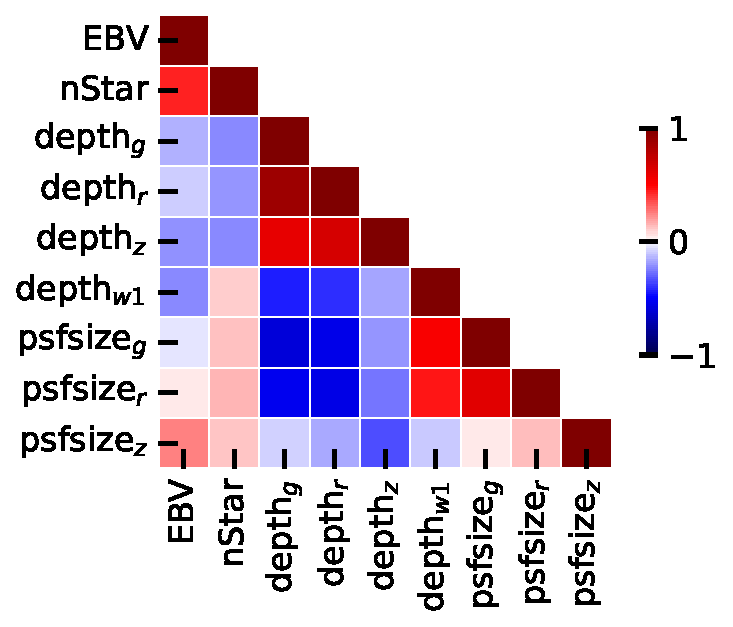
\includegraphics[width=0.5\textwidth]{figures/pccx.pdf}  
 \caption{Top: Pearson correlation coefficients between the DR9 LRG density and imaging properties in the three imaging regions. Solid curves represent the $95\%$ spread of correlation coefficients observed in 100 randomly selected lognormal mock density realizations. Bottom: Pearson correlation matrix from imaging properties for the full DESI footprint.}
 \label{fig:pcc}
\end{figure}



Fig. \ref{fig:pcc} shows the Pearson correlation coefficient between the DR9 LRG density and DESI imaging properties for the three imaging surveys (DECaLS North, DECaLS South, and BASS+MzLS) in the top panel. The horizontal curves are constructed from lognormal simulations (see, subsection \ref{ssec:mocks}) to quantify the significance of correlations. Fig. \ref{fig:pcc} (bottom) shows the correlation matrix among imaging properties for the DESI footprint. There is a strong correlation between the LRG density and depth maps, and next correlated properties seem to be Galactic foregrounds. There is a small correlation between the LRG density and the W1 depth and psfsize properties. We observe a significant inner correlation among the imaging properties themselves, especially between the local stellar density and Milky Way extinction; also, the $r$-band and $g$-band survey properties are more correlated with each other than with the $z$-band. We also investigate the correlations using the Spearman-r correlation, but find no significant differences.

\subsubsection{Imaging weights}
We follow a regression approach to model the spatial dependence of spurious fluctuations in the DR9 density map to the information encoded by the imaging templates. Both linear multivariate and nonlinear regression are applied to assess the level of nonlinear systematic effects. 

Regression analyses are performed separately for each imaging survey as our preliminary analysis indicated that each region responds differently to each template (see, e.g., Fig. \ref{fig:pcc} top panel). The optimal parameters associated with the linear and nonlinear models are found by optimizing the negative Poisson log-likelihood, $\lambda - \rho \log(\lambda)$, between the observed galaxy density $\rho$ and the output predicted density $\lambda$ from the models given imaging properties \textbf{x} as input. We do not provide spatial information as input to avoid subtracting clustering signal. With $\lambda(\textbf{x}) = \log (1+e^{f(\textbf{x})})$, we investigate the use of linear multivariate and nonlinear models to approximate $f$. For the linear model, we perform a Monte Carlo Markov Chain (MCMC) search using the \textsc{emcee} package \citep{2013PASP..125..306F} and all of the DR9 data to calculate the Poisson log-likelihood. 

For the nonlinear approximation, we employ the implementation of artificial neural networks from \cite{rezaie2021primordial}; specifically, the nonlinear model is composed of an ensemble of 20 neural network models. Each neural network consists of imaging maps on the first layer, three hidden layers with 20 rectifier units on each layer, and single unit with the identity function in the output layer. The rectifier is the identity function for positive input and zero for negative, and it introduces nonlinearities in the neural network architecture. Unlike the linear regression, we use $60\%$ of the LRG data for training, $20\%$ for validation, and $20\%$ for testing in order to minimize the chance of over-subtraction, i.e.g, regressing out some of clustering signal by the nonlinear model. However, we are able to test the nonlinear model on the entire LRG data with the technique of permuting the choice of the training, validation, or testing sets. We train the neural networks for up to 70 training epochs with the gradient descent \textsc{Adam} optimizer \citep{2017arXiv171105101L}, i.e., the parameters are updated iteratively following the gradient of the negative Poisson log-likelihood. We initialize the learning rate by minimizing the loss on the validation set and adjust it to dynamically vary between two boundary values of $0.001$ and $0.1$ to avoid local minima during gradient descent. The best neural network model is then selected from the lowest prediction error when applied to the validation set. Finally, we run the ensemble of 20 best-fit models through the test set and average over the predictions to construct the predicted galaxy density map in \textsc{HEALPix}. The predicted galaxy density is normalized and applied as imaging weights to down-weight the observed density map of LRGs to reduce spurious fluctuations in the LRG data. 

Because of the inner correlation amongst the maps (see, e.g., Fig. \ref{fig:pcc} bottom panel), a few subsets of imaging maps are considered as input for more conservative treatment of systematic errors. These subsets are selected to minimize the cross-correlations between the cleaned LRG density field and imaging properties while avoiding highly correlated templates:
\begin{itemize}
\item \textbf{Conservative I}: Extinction and z-band depth
\item \textbf{Conservative II}: Extinction, z-band depth, and r-band psfsize
\item \textbf{All Maps}: Extinction, depth in $grz$ and $W1$, psfsize in $grz$
\end{itemize}

Upon inspecting the predicted density maps, we find that while most of the large-scale spurious fluctuations are explained by just the extinction map and depth in the z band, adding the r-band psfsize results in a finer structure in the predicted density map, and as we show later it reduces the cross-correlation between the LRG density and the z band psfsize. We observe that using all imaging maps as input features for regression does not add more information, as expected due to the strong correlations between different bands. Comparing the weights from the linear model to that of the nonlinear approach for the same input maps, we find that the nonlinear approach yields finer structures due to higher flexibility. Overall consistent with the LRG data, both models predict higher galaxy density near the boundaries where the DESI imaging surveys observed the high extinction regions of the Milky Way. These over-dense regions are likely contaminated artifacts entering the LRG selection, e.g., stellar contaminants or other artifacts because of obscured photometry by MW extinction. The assessment of these imaging weights is further analyzed in \ref{ssec:characterization}. We also investigate the use of all imaging maps as a case which is highly prone to over-subtracting the true clustering signal. Additionally, we assess the robustness of our results against remaining systematic errors by adding external templates for the neutral hydrogen column density \citep{2016A&A...594A.116H} and the photometric calibration (e.g., in the z band; \textit{CALIBZ}). The effects on $\fnl$ constraints are discussed in Section \ref{sec:results}.


\subsection{Synthetic lognormal density fields}\label{ssec:mocks}
Density fluctuations of galaxies on large scales can be approximated with lognormal distributions \citep{coles1991}. Unlike N-body simulations, simulating lognormal density fields is not computationally intensive, and allows quick and robust validation of data analysis pipelines. We use \textsc{FLASK} \citep[Full-sky Lognormal Astro-fields Simulation Kit;][]{Xavier_2016} to generate ensembles of synthetic galaxy density fields that mimic the redshift and angular distributions of the DR9 LRG sample (see, Fig. \ref{fig:nz}). We create 1000 realizations with $\fnl=0$ and $76.92$ using a redshift dependent bias $b(z)=1.43/D(z)$, consistent with \cite{zhou2021clustering}. We adapt the fiducial cosmology from a flat $\Lambda$CDM universe, including one massive neutrino with $m_{\nu}=0.06$ eV, and the rest of cosmological parameters is deducted from Planck 2018 \citep{aghanim2020planck},
\begin{equation*}
 h = 0.67, \Omega_{M}=0.31, \sigma_{8}=0.8, {\rm and}~ n_{s}=0.97.
\end{equation*}
The same cosmology is employed throughout the rest of the manuscript. We demonstrate later in Section \ref{sec:results} that our $\fnl$ constraints are quite robust against the choice of our fiducial cosmology.

\subsubsection{Contaminated mocks}
The linear multivariate model with the templates for the extinction, depth$_{z}$, psfsize$_{r}$ (conservative II) is used to induce observational imaging spurious fluctuations in the lognormal density fields. We choose the linear model for the contamination to assess how much of the clustering signal is removed by applying more flexible models (based on neural networks) for cleaning. The parameters of the linear model are fit on the DR9 LRG sample, separately on each imaging survey. The contamination model is drawn from the posteriors sampled by MCMC, and thus is distinct for each realization of lognormal density field. The same contamination model is applied to both the $\fnl=0$ and $76.92$ mocks.

Similar to the DR9 sample, the linear and nonlinear mitigation methods are applied to the simulations, with and without PNG or with and without the imaging-dependent systematics, to derive the imaging weights. Section \ref{sec:results} presents how we use these mock results to calibrate the amount of the clustering power that is removed by the cleaning methods. We use no prior knowledge regarding the underlying contamination model or the templates used. 